%%%
% Plantilla de Presentación
% Modificación de una plantilla de Latex de LaTeXTemplates para adaptarla 
% al castellano y a las necesidades de escribir informática y matemáticas.
%
% Editada por: Mario Román
%
% License:
% CC BY-NC-SA 3.0 (http://creativecommons.org/licenses/by-nc-sa/3.0/)
%%%

%%%%%%%%%%%%%%%%%%%%%%%%%%%%%%%%%%%%%%%%%
% Beamer Presentation
% LaTeX Template
% Version 1.0 (10/11/12)
%
% This template has been downloaded from:
% http://www.LaTeXTemplates.com
%
% License:
% CC BY-NC-SA 3.0 (http://creativecommons.org/licenses/by-nc-sa/3.0/)
%
%%%%%%%%%%%%%%%%%%%%%%%%%%%%%%%%%%%%%%%%%

%----------------------------------------------------------------------------------------
%	PAQUETES Y CONFIGURACIÓN DEL DOCUMENTO
%----------------------------------------------------------------------------------------

\documentclass{beamer}

%% Configuración de la presentación
\mode<presentation> {
  %%% Selección de estilo
  % The Beamer class comes with a number of default slide themes
  % which change the colors and layouts of slides. Below this is a list
  % of all the themes, uncomment each in turn to see what they look like.

  %\usetheme{default}
  %\usetheme{AnnArbor}
  %\usetheme{Antibes}
  %\usetheme{Bergen}
  %\usetheme{Berkeley}
  %\usetheme{Berlin}
  %\usetheme{Boadilla}
  %\usetheme{CambridgeUS}
  %\usetheme{Copenhagen}
  %\usetheme{Darmstadt}
  %\usetheme{Dresden}
  %\usetheme{Frankfurt}
  %\usetheme{Goettingen}
  %\usetheme{Hannover}
  %\usetheme{Ilmenau}
  %\usetheme{JuanLesPins}
  %\usetheme{Luebeck}
  \usetheme{Madrid}
  %\usetheme{Malmoe}
  %\usetheme{Marburg}
  %\usetheme{Montpellier}
  %\usetheme{PaloAlto}
  %\usetheme{Pittsburgh}
  %\usetheme{Rochester}
  %\usetheme{Singapore}
  %\usetheme{Szeged}
  %\usetheme{Warsaw}

  %% Selección de color
  % As well as themes, the Beamer class has a number of color themes
  % for any slide theme. Uncomment each of these in turn to see how it
  % changes the colors of your current slide theme.

  %\usecolortheme{albatross}
  %\usecolortheme{beaver}
  %\usecolortheme{beetle}
  %\usecolortheme{crane}
  %\usecolortheme{dolphin}
  %\usecolortheme{dove}
  %\usecolortheme{fly}
  %\usecolortheme{lily}
  %\usecolortheme{orchid}
  %\usecolortheme{rose}
  %\usecolortheme{seagull}
  %\usecolortheme{seahorse}
  %\usecolortheme{whale}
  %\usecolortheme{wolverine}

  %% Configuración del pie de línea
  %\setbeamertemplate{footline} % To remove the footer line in all slides uncomment this line
  %\setbeamertemplate{footline}[page number] % To replace the footer line in all slides with a simple slide count uncomment this line
  %\setbeamertemplate{navigation symbols}{} % To remove the navigation symbols from the bottom of all slides uncomment this line
}

%% Fuentes de tamaño arbitrario
\usepackage{lmodern}

%% Gráficos
\usepackage{graphicx} % Allows including images
\usepackage{booktabs} % Allows the use of \toprule, \midrule and \bottomrule in tables

%%% Castellano.
% noquoting: Permite uso de comillas no españolas.
% lcroman: Permite la enumeración con numerales romanos en minúscula.
% fontenc: Usa la fuente completa para que pueda copiarse correctamente del pdf.
\usepackage[spanish,es-noquoting,es-lcroman]{babel}
\usepackage[utf8]{inputenc}
\usepackage[T1]{fontenc}
\selectlanguage{spanish}
\unaccentedoperators

% Algoritmos
\usepackage{algorithm}
\usepackage{algpseudocode}

%----------------------------------------------------------------------------------------
%	TÍTULO
%----------------------------------------------------------------------------------------

\title[Primalidad en Tiempo Polinomial]{Primalidad en Tiempo Polinomial} % The short title appears at the bottom of every slide, the full title is only on the title page

\author{Francisco Gallego Salido} % Your name
\institute[UGR] % Your institution as it will appear on the bottom of every slide, may be shorthand to save space
{
  Universidad de Granada \\ % Your institution for the title page
  \medskip
  \textit{fgallego@correo.ugr.es} % Your email address
}
\date{\today} % Date, can be changed to a custom date



\begin{document}

%% Diapositiva de título.
\begin{frame}
\titlepage % Print the title page as the first slide
\end{frame}

%% Diapositiva de contenidos.
% Throughout your presentation, if you choose to use \section{} and \subsection{} commands, 
% these will automatically be printed on this slide as an overview of your presentation
\begin{frame}
  \frametitle{Contenidos} % Table of contents slide, comment this block out to remove it
  \tableofcontents
\end{frame}



%----------------------------------------------------------------------------------------
%	PRESENTACIÓN
%----------------------------------------------------------------------------------------

\section{Tests de Primalidad}

\begin{frame}
	\centering
	\begin{Huge}
		Tests de Primalidad
	\end{Huge}
\end{frame}

\subsection{Introducción}

\begin{frame}{¿Qué es un test de primalidad?}
	Un test de primalidad es un algoritmo que nos permite determinar si un número es primo o no.\break
	
	El test más básico es el que se deriva de la definición de primalidad, cuya complejidad es $O(\sqrt{n})$:
	
	\begin{itemize}[<+(1)->]
		\item Comprobar todos los números menores que $\lfloor\sqrt{n}\rfloor$ y ver si alguno divide a $n$.
		
		\item Si ninguno lo divide, $n$ es primo.
		
		\item Si alguno lo divide, $n$ es compuesto.
	\end{itemize}
\end{frame}

\subsection{Pequeño Teorema de Fermat}

\begin{frame}{Pequeño Teorema de Fermat}
	\onslide<1->Un test mucho más eficiente es el que se deriva del \textit{Pequeño Teorema de Fermat}.\break
	
	\onslide<2->
	\begin{theorem}[Pequeño Teorema de Fermat]
		Si $n$ es primo, entonces $a^n \equiv a \mod(n)$ para todo $a \in \mathbb{Z}$.
	\end{theorem}
	
	\onslide<3->El test consiste en comprobar varios valores de $a$ y vemos si se cumple la congruencia.\break
	
	\onslide<4->Si falla para algún $a$, entonces $n$ es compuesto. En caso contrario, $n$ probablemente sea primo.
\end{frame}

\begin{frame}{Problema}
	\onslide<1->No es cierto en general que si $a^n \equiv a \mod(n)$ para todo $a \in \mathbb{Z}$, entonces $n$ sea primo.\break
	
	\onslide<2->Los \textit{Números de Charmichael} son contraejemplos de ello, donde $561 = 3\cdot11\cdot17$ es el primer elemento de dicho conjunto.
\end{frame}

\section{Algoritmo AKS}

\begin{frame}
	\centering
	\begin{Huge}
		Algoritmo AKS
	\end{Huge}
\end{frame}

\subsection{Introducción}

\begin{frame}
	Se trata del primer test de primalidad que cumple todas las propiedades deseadas:\break
	
	\begin{itemize}[<+(1)->]
		\item \textbf{General}. Válido para todos los enteros.
		
		\item \textbf{Determinista}. Determina con probabilidad $100\%$ si un número es primo o compuesto.
		
		\item \textbf{Polinómico}. La complejidad asintótica es polinómica en la cantidad de dígitos.
		
		\item \textbf{Incondicional}. No depende de hipótesis no probadas aún.
	\end{itemize}
\end{frame}

\begin{frame}{Idea Principal}
	\onslide<1->El \textit{Pequeño Teorema de Fermat} no proporciona un test válido, pero una versión general suya sí. Sea el siguiente teorema:\break
	
	\onslide<2->
	\begin{theorem}
		Sea $n > 1$ y $a \in \mathbb{Z}$. Entonces $n$ es primo si, y solo si, se cumple
		
		\begin{equation*}
		(X + a)^n \equiv X^n + a \mod(n)
		\end{equation*}
	\end{theorem}
	
	\onslide<3->Un test que se deriva de esta propiedad es simplemente comprobar si la congruencia se cumple para algún $a$.
\end{frame}

\begin{frame}{¿Es este test polinómico?}
	\onslide<1->Este test implica evaluar $n$ coeficientes, luego la complejidad sería $\Omega(n)$.\break
	
	\onslide<2->¿Podemos reducir el número de coeficientes a evaluar?
\end{frame}

\begin{frame}{Solución}
	\onslide<1->Si la congruencia anterior la evaluamos módulo $(X^r - 1, n)$ para algún $r$ escogido apropiadamente, podremos reducir el número de coeficientes. Sea pues la siguiente congruencia:\break
	
	\onslide<2->
	\begin{equation*}
	(X + a)^n \equiv X^n + a \mod(X^r - 1, n)
	\end{equation*}
\end{frame}

\begin{frame}{Nuevo Problema}
	\onslide<1->Esta nueva congruencia sigue siendo cierta cuando $n$ es primo.\break
	
	\onslide<2->No obstante, algunos números compuestos también la cumplen para algunos valores de $r$ y $a$.
\end{frame}

\begin{frame}{Nueva Solución}
	\onslide<1->Esta propiedad se puede reestablecer casi por completo.\break
	
	\onslide<2->Eligiendo $r$ adecuadamente, si la congruencia se cumple para varios valores de $a$, entonces podemos asegurar que $n$ es una potencia de un primo.
\end{frame}

\subsection{El Algoritmo}

\begin{frame}
	\centering
	\begin{Large}
		El Algoritmo
	\end{Large}
\end{frame}

\begin{frame}[fragile]{Pasos del Algoritmo AKS}
	\begin{algorithm}[H]
		\caption{AKS}
		\begin{algorithmic}
			\Procedure{IsPrime}{$n$}\Comment{Comprobar si $n > 1$ es un número primo}
				\State \textbf{if} $n = a^b$ con $a, b > 1$ \Return{COMPUESTO}\Comment{Paso 1}\medskip
				\State Encontrar el menor $r$ tal que $ord_r(n) > \log^2(n)$.\Comment{Paso 2}\medskip
				\State \textbf{if} $1 < (a, n) < n$ para algún $a \leq r$ \Return{COMPUESTO}\Comment{Paso 3}\medskip
				\State \textbf{if} $n \leq r$ \Return{PRIMO}\Comment{Paso 4}\medskip
				\For{$a = 1$ hasta $\lfloor \sqrt{\phi(r)}\log(n) \rfloor$}\Comment{Paso 5}
					\State \textbf{if} $(X + a)^n \not\equiv X^n + a \mod(n, X^r - 1)$ \Return{COMPUESTO}
				\EndFor\medskip
				\State \Return{PRIMO}\Comment{Paso 6}
			\EndProcedure
		\end{algorithmic}
	\end{algorithm}
\end{frame}

\begin{frame}{Ejemplo}
	Sea el número $31$, el cual ya sabemos que es primo.
	
	\begin{enumerate}[<+(1)->]
		\item $31$ no es una potencia perfecta. Pasamos al siguiente paso.
		
		\item El menor $r$ es $29$, pues $ord_{29}(31) = 28 > \log^2(31) \simeq 24.54$.
		
		\item $(a, 31) = 1$ para todo $a \leq 29$. Pasamos al siguiente paso.
		
		\item $31 \not\leq 29$. Pasamos al siguiente paso.
		
		\item
		
		\begin{itemize}
			\item $\lfloor\sqrt{\phi(r)}\log(n)\rfloor = 26$.
			
			\item $(X + a)^{31} = x^2 + a^{31}$ módulo $(X^{29}-1, 31)$.
			
			\item $X^{31} + a = x^2 + a$ módulo $(X^{29}-1, 31)$.
			
			\item $a^{31} \equiv a \mod(X^{29}-1, 31)$ para todo $1 \leq a \leq 26$. Pasamos al siguiente paso
		\end{itemize}
		
		\item Hemos llegado al último paso, por lo que $31$ es primo.
	\end{enumerate}
\end{frame}

\subsection{Complejidad}

\begin{frame}
	\centering
	\begin{Large}
		Complejidad
	\end{Large}
\end{frame}

\begin{frame}{Valor de $r$}
	\onslide<1->El valor encontrado en el segundo paso es crucial para que el test sea polinómico.\break
	
	\onslide<2->De dicho valor dependen la complejidad del paso $5$.\break
	
	\onslide<3->Dicho valor se puede probar que está acotado por $\max\{3, \lceil\log^5(n)\rceil\}$.
\end{frame}

\begin{frame}{Complejidad Paso a Paso}
	\onslide<1->Cada paso tiene un complejidad determinada:\break
	
	\onslide<2->
	\begin{itemize}
		\item $O^\sim(\log^3(n))$.
		\item $O^\sim(\log^7(n))$.
		\item $O^\sim(\log^6(n))$.
		\item $O(\log(n))$.
		\item $O^\sim(\log^{21/2}(n))$.
		\item $O(1)$.
	\end{itemize}
\end{frame}

\begin{frame}{Complejidad Quinto Paso}
	\onslide<1->Hay que comprobar $O(r^{1/2}\log(n))$ congruencias polinómicas.\break
	
	\onslide<2->Cada congruencia consiste de $O(\log(n))$ multiplicaciones de polinomios de grado $O(r)$ con coeficientes de tamaño $O(\log(n))$.\break
	
	\onslide<3->Esto produce una complejidad asintótica de $O^\sim(r^{3/2}\log^3(n))$, que teniendo que $r = O(\log^5(n))$, nos queda finalmente $O^\sim(\log^{21/2}(n))$.
\end{frame}

\begin{frame}{Complejidad Total}
	\onslide<1->La complejidad del quinto paso es la más alta, luego el algoritmo \textbf{AKS} tiene una complejidad algorítmica de $O^\sim(\log^{21/2}(n))$.\break
	
	\onslide<2->Usando \textit{Teoría de Cribas} se puede probar que $r = O(\log^3(n))$, reduciendo la complejidad hasta $O^\sim(\log^{15/2}(n))$.\break
	
	\onslide<3->Bajo ciertas hipótesis no probadas (como puede ser la \textit{Hipótesis Generalizada de Riemann}), se puede probar que $r = O(\log^2(n))$, reduciendo una vez más la complejidad hasta $O^\sim(\log^6(n))$.
\end{frame}

\section{Comparaciones}

\begin{frame}
	\centering
	\begin{Huge}
		Implementación y Análisis
	\end{Huge}
\end{frame}

\subsection{Test AKS}

\begin{frame}{Detalles del test AKS}
	\onslide<1->Hay varias consideraciones para el test AKS:
	
	\onslide<2->
	\begin{itemize}
		\item Es importante usar buena multiplicación de polinomios. De lo contrario el test es inservible en la práctica.
		
		\item Calcular cotas lo más fieles posibles.
		
		\item Utilizar enteros de precisión arbitraria.
	\end{itemize}
	
	\onslide<3->Utilizar un lenguaje de programación rápido. como puede ser C++
\end{frame}

\subsection{Tests Probabilísticos}

\subsubsection{Test de Miller-Rabin}

\begin{frame}{Test de Miller-Rabin}
	Test probabilístico basado en las siguientes congruencias aplicables a enteros mayores que $2$ impares para varias bases $a$:\break
	
	\onslide<2->
	\begin{align}
	a^d &\equiv 1 \mod(n)\\
	a^{2^r d} &\equiv -1 \mod(n)\text{ con $0 \leq r < s$,}
	\end{align}
	
	donde $n = 2^rd + 1$ con $d \geq 1$ impar y $r \geq 1$.
\end{frame}

\subsubsection{Test de Solovay-Strassen}

\begin{frame}{Test de Solovay-Strassen}
	Test probabilístico basado en la siguiente congruencia relacionada con el \textit{Símbolo de Jacobi}, la cual se cumple para los primos:\break
	
	\onslide<2->
	\begin{equation}
	a^{\frac{(n-1)}{2}} \equiv \left(\frac{a}{n}\right) \mod(n),
	\end{equation}
\end{frame}

\begin{frame}{Estructura}
	\begin{alertblock}{}
		\begin{center}
			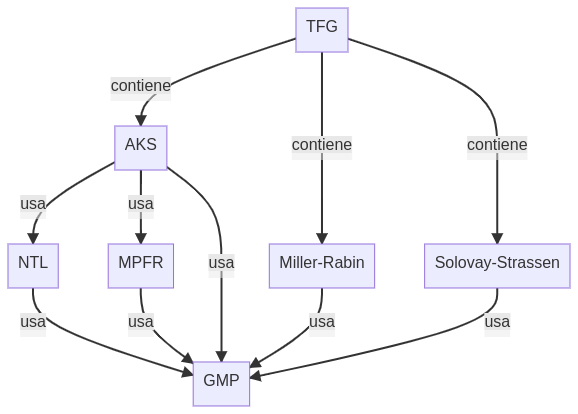
\includegraphics[scale=0.40]{../Memoria/img/diagrama-relaciones}
		\end{center}
	\end{alertblock}
\end{frame}

\subsection{Comparaciones}

\begin{frame}
	\begin{Large}
		Comparaciones
	\end{Large}
\end{frame}

\begin{frame}{Comparación Números Primos}
	\onslide<1->
	Mayores primos que ocupan $n$ bits. Por ejemplo, el $7$ es el mayor primo con $3$ bits, $31$ el mayor primo con $5$ bits, etc.
	
	\onslide<2->
	\begin{alertblock}{}
		\begin{center}
			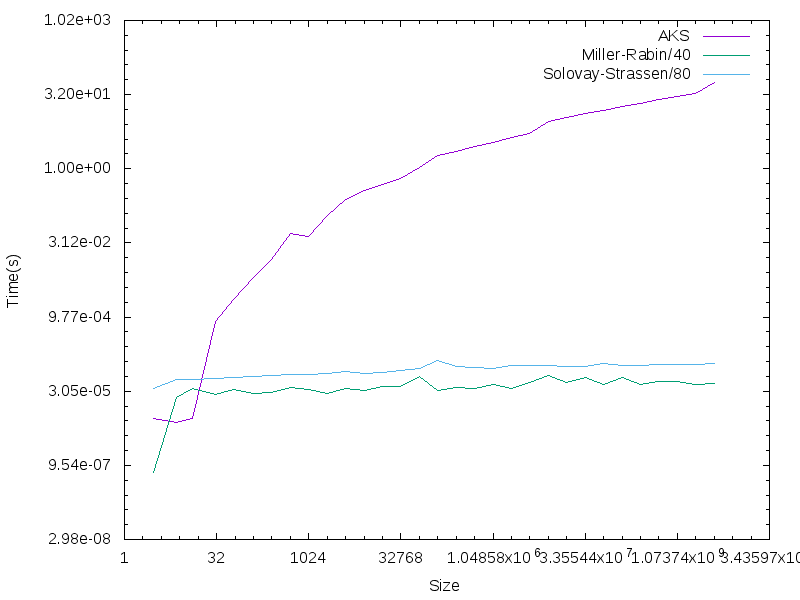
\includegraphics[scale=0.40]{../Memoria/img/graphs/aks-probs-primes-mean}
		\end{center}
	\end{alertblock}
\end{frame}

\begin{frame}{Comparación Potencias Perfectas}
	\onslide<1->
	\begin{itemize}
		\item \textbf{Izquierda}. Primos de hasta $16$ bits elevados a $100$.
		
		\item \textbf{Derecha}. Primos de entre $192$ y $256$ bits elevados a $5$.
	\end{itemize}
	
	\onslide<2->
	\begin{alertblock}{}
		\begin{center}
			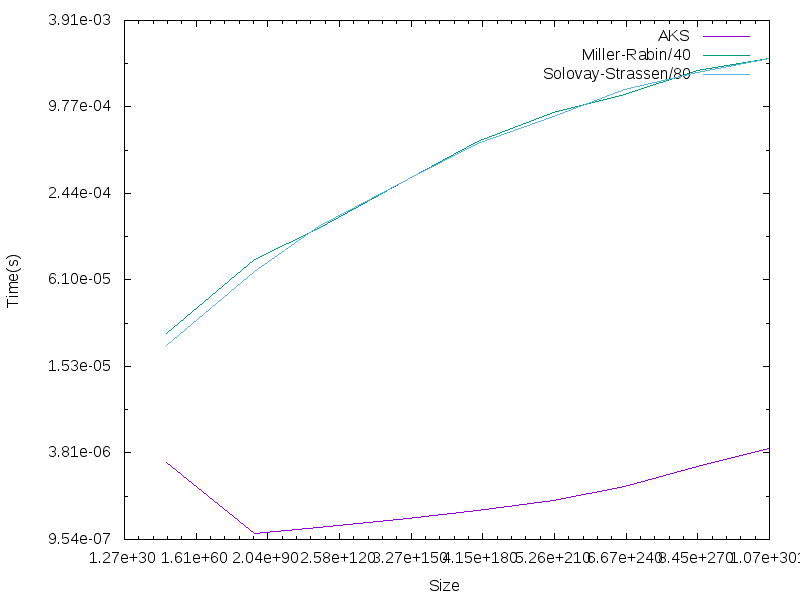
\includegraphics[scale=0.27]{../Memoria/img/graphs/aks-probs-powers-100-mean}
			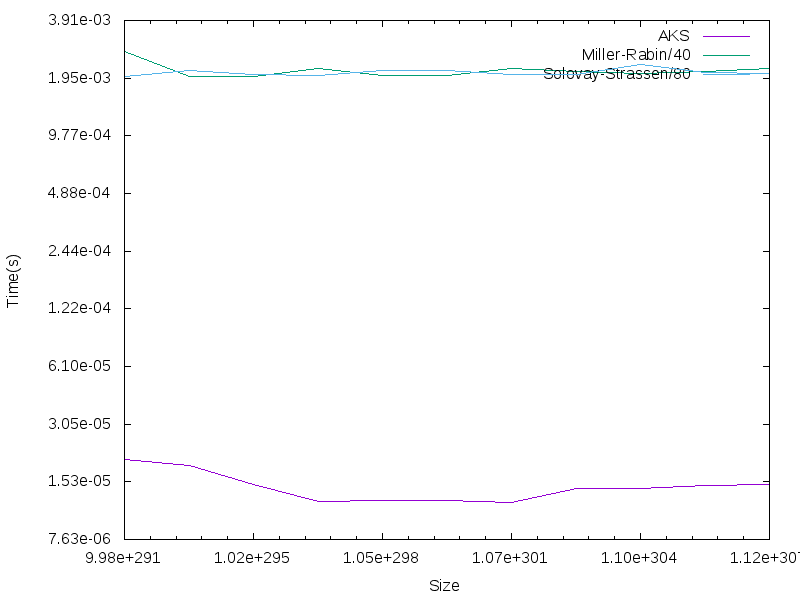
\includegraphics[scale=0.27]{../Memoria/img/graphs/aks-probs-powers-5-mean}
		\end{center}
	\end{alertblock}
\end{frame}

\begin{frame}{Comparación Compuestos No Potencias Perfectas}
	\onslide<1->
	\begin{itemize}
		\item \textbf{Izquierda}. Primos de entre $32$ y $42$ bits multiplicados por un primo de $16$ bits.
		
		\item \textbf{Derecha}. Primos de entre $32$ y $42$ bits multiplicados por un primo de $32$ bits.
	\end{itemize}
	
	\onslide<2->
	\begin{alertblock}{}
		\begin{center}
			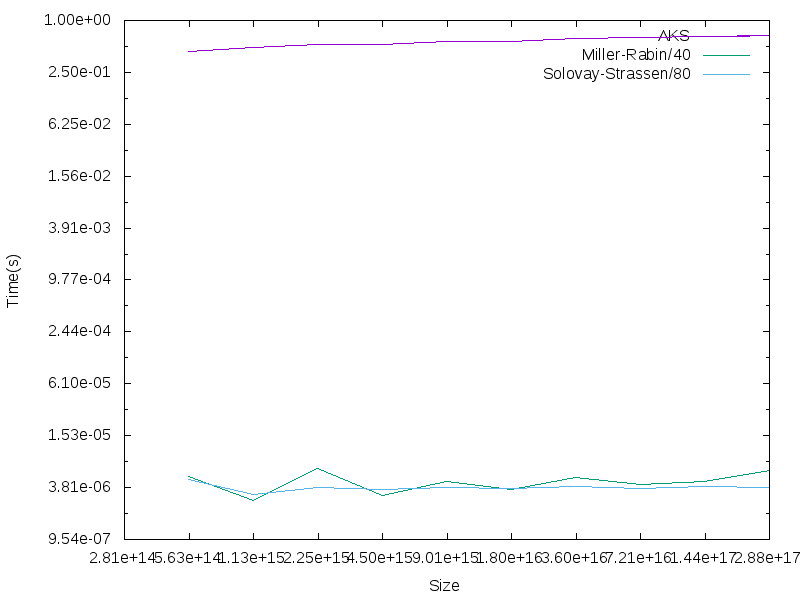
\includegraphics[scale=0.27]{../Memoria/img/graphs/aks-probs-comps-16-mean}
			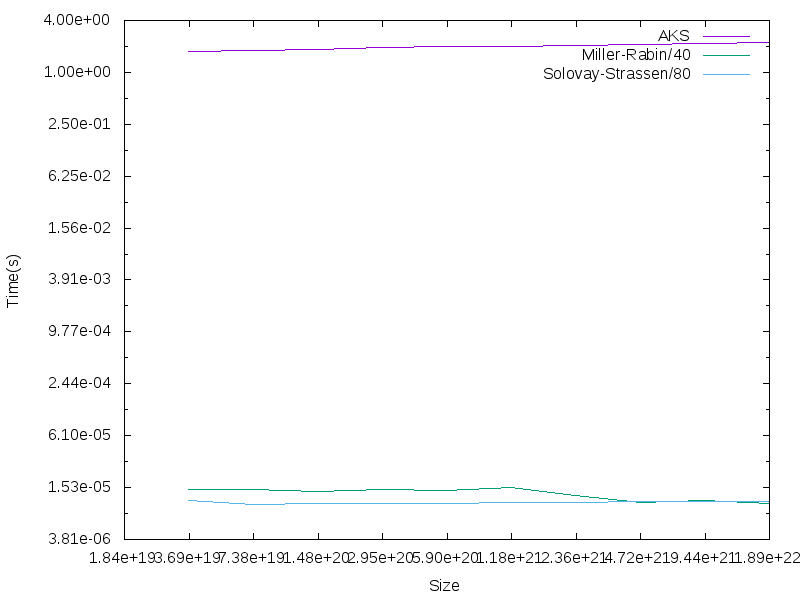
\includegraphics[scale=0.27]{../Memoria/img/graphs/aks-probs-comps-32-mean}
		\end{center}
	\end{alertblock}
\end{frame}

\section{Conclusiones}

\begin{frame}
	\centering
	\begin{Huge}
		Conclusiones
	\end{Huge}
\end{frame}

\begin{frame}{Conclusiones}
	\onslide<1->El test es brillante desde el punto de vista matemático, ya que la prueba de la validez del test usa herramientas elementales.\break
	
	\onslide<2->Sin embargo, a pesar de ser un test polinómico, en la práctica queda muy por detrás de otros test usados en la actualidad.
\end{frame}

%------------------------------------------------

%% Bibliografía
\begin{frame}
\frametitle{Referencias}
\footnotesize{
	\begin{thebibliography}{99} % Beamer does not support BibTeX so references must be inserted manually as below
		\bibitem[AKS04a]{AKS2004}
		Manindra Agrawal, Neeraj Kayal, and Nitin Saxena.
			\newblock {PRIMES} is in {P}.
			\newblock {\em Ann. of Math. (2)}, 160(2):781--793, 2004.
		\bibitem[AKS19]{AKS2019}
		Manindra Agrawal, Neeraj Kayal, and Nitin Saxena.
			\newblock Errata: {PRIMES} is in {P}.
			\newblock {\em Ann. of Math. (2)}, 189(1):317--318, 2019.
		\bibitem[Sal]{fgallego_tfg_github}
		Francisco~Gallego Salido.
			\newblock Tfg.
			\newblock \url{https://github.com/fgallegosalido/TFG}.
	\end{thebibliography}
}
\end{frame}

%------------------------------------------------

\begin{frame}
\Huge{\centerline{Fin}}
\end{frame}

%----------------------------------------------------------------------------------------

\end{document} 